%=============================================================================
%  Note technique -- Evaluation de NVIDIA-NemotronLabs-VoiceChat-11B
%  Projet : Simulateur de controleur aerien -- copilote IA pour le controle aerien
%  Auteur : Nicolas Marano -- URCA / supercalculateur ROMEO (NVIDIA GH200)
%  Compilation : pdflatex (x2 pour la table des matieres) -- voir build.sh
%=============================================================================
\documentclass[11pt,a4paper]{article}

\usepackage[utf8]{inputenc}
\usepackage[T1]{fontenc}
\usepackage[french]{babel}
\usepackage{lmodern}
\usepackage{microtype}
\usepackage[a4paper,margin=2.3cm,headheight=15pt]{geometry}
\usepackage{graphicx}
\usepackage{booktabs}
\usepackage{array}
\usepackage[table]{xcolor}
\usepackage[nobottomtitles*]{titlesec}
\usepackage{enumitem}
\usepackage{caption}
\usepackage{fancyhdr}
\usepackage{listings}
\usepackage[most]{tcolorbox}
\usepackage{hyperref}

%--- Couleurs (identiques aux rapports du projet) -----------------------------
\definecolor{atcblue}{RGB}{11,61,145}
\definecolor{atcteal}{RGB}{13,110,124}
\definecolor{atcgreen}{RGB}{22,128,71}
\definecolor{atcred}{RGB}{197,32,38}
\definecolor{atcpurple}{RGB}{109,40,180}
\definecolor{atcslate}{RGB}{71,85,105}
\definecolor{lightgray}{RGB}{244,246,249}
\definecolor{rulegray}{RGB}{210,216,224}

\hypersetup{colorlinks=true, linkcolor=atcblue, urlcolor=atcteal, citecolor=atcblue,
  pdftitle={Note technique -- VoiceChat-11B sur la tache ATC},
  pdfauthor={Nicolas Marano}}

\titleformat{\section}{\Large\bfseries\color{atcblue}}{\thesection}{0.6em}{}
\titleformat{\subsection}{\large\bfseries\color{atcteal}}{\thesubsection}{0.6em}{}
\titleformat{\subsubsection}{\normalsize\bfseries\color{atcteal}}{\thesubsubsection}{0.5em}{}
\titlespacing*{\section}{0pt}{16pt}{8pt}
% chaque grande section demarre sur une nouvelle page
\newcommand{\sectionbreak}{\clearpage}
\renewcommand{\bottomtitlespace}{0.12\textheight}
% jamais de ligne veuve ni orpheline
\widowpenalty=10000
\clubpenalty=10000
\displaywidowpenalty=10000

\pagestyle{fancy}
\fancyhf{}
\renewcommand{\headrulewidth}{0.4pt}
\renewcommand{\footrulewidth}{0.4pt}
\fancyhead[L]{\small\color{atcblue}\itshape Copilote IA pour le contrôle aérien}
\fancyhead[R]{\small\color{atcblue}\itshape Note technique : VoiceChat-11B}
\fancyfoot[L]{\small Nicolas Marano, URCA / ROMEO}
\fancyfoot[R]{\small\thepage}

\newtcolorbox{objbox}{enhanced, colback=lightgray, colframe=atcblue,
  boxrule=0.8pt, arc=3pt, left=10pt, right=10pt, top=8pt, bottom=8pt,
  fonttitle=\bfseries\color{white}, coltitle=white, colbacktitle=atcblue,
  title={Question posée}}

\newtcolorbox{resbox}{enhanced, colback=atcgreen!6, colframe=atcgreen,
  boxrule=0.8pt, arc=3pt, left=10pt, right=10pt, top=8pt, bottom=8pt,
  fonttitle=\bfseries, coltitle=white, colbacktitle=atcgreen,
  title={Résultats clés}}

\newtcolorbox{warnbox}{enhanced, colback=atcslate!6, colframe=atcslate,
  boxrule=0.8pt, arc=3pt, left=10pt, right=10pt, top=8pt, bottom=8pt,
  fonttitle=\bfseries, coltitle=white, colbacktitle=atcslate,
  title={Contraintes techniques et choix d'ingénierie}}

\newtcolorbox{redbox}{enhanced, colback=atcred!5, colframe=atcred,
  boxrule=0.8pt, arc=3pt, left=10pt, right=10pt, top=8pt, bottom=8pt,
  fonttitle=\bfseries, coltitle=white, colbacktitle=atcred,
  title={Limite bloquante identifiée}}

\lstdefinestyle{atccode}{
  basicstyle=\ttfamily\footnotesize,
  backgroundcolor=\color{lightgray},
  frame=single, framesep=5pt, rulecolor=\color{rulegray},
  breaklines=true, breakatwhitespace=true,
  showstringspaces=false,
  keywordstyle=\color{atcblue}\bfseries,
  commentstyle=\color{atcgreen}\itshape,
  stringstyle=\color{atcpurple},
  columns=fullflexible, keepspaces=true,
  aboveskip=8pt, belowskip=8pt,
}
\lstset{style=atccode}

\setlist[itemize]{label=\textbullet, leftmargin=1.4em, itemsep=2pt, topsep=3pt}
\captionsetup{font=small, labelfont={bf,color=atcblue}}
% legendes : au-dessus pour les tableaux, en dessous pour les figures
\captionsetup[table]{position=top, skip=6pt}
\renewcommand{\arraystretch}{1.25}

%=============================================================================
\begin{document}

%--- Page de garde -----------------------------------------------------------
\begin{titlepage}
\centering
\vspace*{1.2cm}
{\color{atcblue}\rule{\textwidth}{2pt}}\\[0.5cm]
{\Huge\bfseries\color{atcblue} Note technique d'évaluation\par}
\vspace{0.35cm}
{\LARGE\color{atcteal} Un modèle parole-à-parole bout-en-bout\\ peut-il remplacer la cascade STT $\rightarrow$ LLM $\rightarrow$ TTS ?\par}
\vspace{0.25cm}
{\large Évaluation de \texttt{nvidia/NVIDIA-NemotronLabs-VoiceChat-11B}\\[2pt]
sur les clairances du banc de benchmark du projet\par}
\vspace{0.4cm}
{\color{atcblue}\rule{\textwidth}{2pt}}\\[1.0cm]

{\large\itshape Un copilote d'intelligence artificielle pour le contrôle aérien\par}
\vspace{1.4cm}

{\normalsize
\begin{tabular}{rl}
\large\bfseries Auteur & \large Nicolas Marano\\[4pt]
\large\bfseries Projet & \large Simulateur de contrôleur aérien (PoC)\\[4pt]
\large\bfseries Établissement & \large Université de Reims Champagne-Ardenne (URCA)\\[4pt]
\large\bfseries Calcul & \large Supercalculateur ROMEO : GH200 120\,Go (aarch64)\\[4pt]
\large\bfseries Date de la campagne & \large 19 août 2026\\[4pt]
\large\bfseries Nature & \large Test exploratoire (hors périmètre du rapport final)\\
\end{tabular}}

\vfill
\begin{tcolorbox}[colback=lightgray, colframe=atcblue, arc=3pt, width=0.94\textwidth, center,
  left=12pt, right=12pt, top=8pt, bottom=8pt]
\small\centering
\textbf{Résumé.} Le projet repose sur une \emph{cascade} de trois services
(reconnaissance vocale, LLM, synthèse). NVIDIA a publié le 3 août 2026 un modèle
\emph{bout-en-bout} full-duplex de 11--12 milliards de paramètres qui réalise les
trois fonctions en un seul réseau, avec appel d'outils. Cette note mesure ce que
donne ce modèle sur la tâche du projet, en comparaison \textbf{appariée} avec la
cascade déjà évaluée sur le même calculateur. Résultat : le modèle comprend
l'\emph{instruction} dans 66\,\% des cas mais échoue sur les \emph{indicatifs}
OACI, n'émet \textbf{aucun} appel d'outil sur 100 essais, et reste
significativement en retrait de la cascade (McNemar apparié,
$p_{\text{Holm}} \le 0{,}008$). En revanche sa voix de synthèse est la plus
intelligible de toutes celles mesurées dans le projet.
\end{tcolorbox}
\vspace{0.6cm}
{\small Année universitaire 2025--2026}
\end{titlepage}

\tableofcontents
\thispagestyle{fancy}
\vspace{0.8cm}

%=============================================================================
\section{Objet du test et positionnement}
%=============================================================================

\begin{objbox}
L'architecture du projet est une \textbf{cascade} : la parole du contrôleur est
transcrite (Whisper affiné par LoRA sur de l'ATC), la transcription est
interprétée par un LLM (Mistral-7B) en un ordre \texttt{TrafScript} validé, puis
le collationnement du pilote est synthétisé (XTTS ou Kokoro). Trois modèles,
trois appels réseau, trois sources d'erreur cumulées.

NVIDIA propose l'approche exactement opposée. La question est simple :
\textbf{ce modèle unique fait-il aussi bien, sur nos clairances, que nos trois
modèles chaînés ?}
\end{objbox}

\subsection{Deux façons de faire parler une machine}

Pour situer l'enjeu, il faut d'abord rappeler comment fonctionne la chaîne
actuelle. Quand l'élève contrôleur parle dans son micro, trois programmes se
relaient. Le premier, la \emph{reconnaissance vocale} (souvent abrégée STT, pour
\emph{speech-to-text}), écoute l'enregistrement et écrit ce qu'il a entendu :
c'est un modèle Whisper~\cite{whisper} que nous avons spécialisé sur de la
radio aéronautique par la méthode LoRA~\cite{lora}. Le deuxième, un \emph{grand modèle de langage} (LLM), lit cette
transcription et la transforme en une commande que le simulateur sait exécuter,
par exemple \texttt{HDG AFR1234 270} pour un virage au cap 270, ordre que le
simulateur de trafic BlueSky~\cite{bluesky} exécute. Le troisième, la
\emph{synthèse vocale} (TTS, pour \emph{text-to-speech}), lit à voix haute le
collationnement du pilote. Trois modèles, trois appels réseau, et surtout trois
occasions de se tromper qui s'additionnent : c'est ce qu'on appelle une
architecture en \textbf{cascade}.

L'approche \textbf{bout-en-bout} propose l'inverse : un réseau unique qui reçoit
du son et produit du son, sans jamais repasser par du texte intermédiaire.
L'intérêt est évident sur le papier, puisqu'on supprime deux passages de relais
et les erreurs qu'ils introduisent. La difficulté l'est tout autant : ce réseau
doit apprendre en même temps à entendre, à comprendre et à parler, alors que
chaque brique de la cascade peut être entraînée et corrigée séparément. Savoir
laquelle des deux approches gagne sur une tâche donnée est une question
empirique, et c'est précisément ce que cette note tranche pour la nôtre.

\subsection{Le modèle évalué}

\texttt{NVIDIA-NemotronLabs-VoiceChat-11B}~\cite{voicechat11b} (publié le
3 août 2026, licence OpenMDW 1.1, « \emph{ready for research purposes only} ») est un modèle
conversationnel \textbf{full-duplex}. Le terme mérite d'être explicité : un
modèle classique fonctionne comme un talkie-walkie, il écoute, puis réfléchit,
puis parle, chacun son tour ; un modèle full-duplex écoute et parle en même
temps, comme deux personnes au téléphone qui peuvent s'interrompre. Son
architecture réunit un encodeur de parole Fast Conformer~\cite{fastconformer},
une dorsale Nemotron Nano v2 de 9 milliards de paramètres~\cite{nemotronnano2}
(une architecture hybride qui remplace la plupart des couches d'attention par
des couches à espace d'états~\cite{mamba2}), un décodeur de synthèse vocale, et surtout un
\textbf{canal de sortie séparé dédié aux appels d'outils}. D'après NVIDIA,
c'est le premier modèle full-duplex ouvert à en disposer.

Une précaution s'impose sur les sources. Le modèle lui-même n'est documenté que
par sa carte de modèle~\cite{voicechat11b}, qui est un document de
constructeur et non une publication évaluée par les pairs. Les travaux relus
les plus proches sont la description de l'agent vocal full-duplex dont il
dérive~\cite{casanova2025asru} et la méthode de modélisation duplex qui le
sous-tend~\cite{salmduplex}. Les chiffres de performance cités dans cette
section proviennent de la carte de modèle et doivent donc être lus comme des
annonces du constructeur, ce qui est précisément une raison de les vérifier
soi-même.

Ce canal d'outils demande lui aussi une explication, car c'est lui qui rend le
modèle intéressant pour nous. Un \emph{appel d'outil} (\emph{function calling})
est un second canal de sortie par lequel le modèle n'émet pas de la parole mais
une instruction structurée destinée à un autre programme, un peu comme un
serveur qui parle au client tout en transmettant sa commande en cuisine. Appliqué
à notre tâche, cela signifie que le modèle pourrait produire l'ordre destiné au
simulateur \emph{pendant} que sa voix prononce le collationnement, ce qui
supprimerait d'un seul coup les étages de reconnaissance et d'interprétation.

Les chiffres publiés par NVIDIA laissent toutefois entrevoir la difficulté :
une latence de prise de parole de 448\,ms et une précision de sélection d'outil
de 82,5\,\%, mais une précision des \emph{arguments} de seulement 44,2\,\% sur
le banc Full-Duplex-Bench~\cite{fullduplexbench}, dans sa version~v3 consacrée
à l'appel d'outils~\cite{fullduplexbenchv3}. Autrement dit, le modèle choisit assez bien
\emph{quel} outil appeler, mais se trompe une fois sur deux sur les valeurs
qu'il lui passe, ce qui est exactement ce dont nous avons besoin (un cap, un
niveau de vol). La carte du modèle précise également qu'il « n'est pas adapté
aux environnements bruités ou fortement réverbérants ». Notre condition radio,
qui applique un passe-bande VHF de 300 à 3400\,Hz et ajoute un bruit à 12\,dB de
rapport signal/bruit, est donc volontairement adverse : nous testons le modèle
là où son concepteur annonce qu'il est faible, parce que c'est là que se trouve
notre cas d'usage réel.

\subsection{Ce que cette note cherche à établir}

Trois questions sont posées, dans cet ordre. La première est la question
d'architecture : sur nos clairances, un modèle unique fait-il aussi bien que nos
trois modèles chaînés ? La deuxième est une question de faisabilité : le canal
d'appel d'outils, qui est l'argument décisif de ce modèle pour notre usage,
fonctionne-t-il réellement sur une tâche aussi contrainte que la phraséologie
aéronautique ? La troisième est une question de coût : que faut-il consentir, en
mémoire, en temps de calcul et en effort de déploiement, pour obtenir une
réponse aux deux premières ?

Il faut préciser le statut de ce travail. Il s'agit d'un test exploratoire, mené
en marge du périmètre du rapport final, sur un modèle publié seize jours avant la
campagne. Son résultat principal est négatif : le modèle ne remplace pas la
chaîne existante. Un résultat négatif obtenu proprement garde pourtant sa valeur,
à condition d'être établi et non supposé. C'est pourquoi la comparaison est
appariée cas par cas, testée statistiquement, et pourquoi les conditions de
mesure sont décrites assez précisément pour être rejouées. La note documente
aussi, chemin faisant, deux choses réutilisables indépendamment du verdict : la
manière de faire tourner un modèle de 44\,Go sur un calculateur dont les quotas
disque sont saturés, et une contrainte de conception des modèles full-duplex que
la documentation du constructeur passe sous silence.

%=============================================================================
\section{Mise en œuvre sur ROMEO}
%=============================================================================

Le déploiement a représenté l'essentiel de l'effort : environ deux jours pour
faire tourner le modèle, contre une heure pour la campagne elle-même. Il est
documenté ici parce que les obstacles rencontrés ne sont pas propres à ce
modèle et se reposeront à l'identique pour toute campagne lourde sur ce
calculateur.

Deux notions suffisent à lire ce qui suit. Un \emph{checkpoint} est le fichier
qui contient les poids appris du modèle, c'est-à-dire le modèle lui-même une
fois entraîné ; celui de VoiceChat pèse 44,4\,Go. Un \emph{quota} est la place
disque qu'un utilisateur a le droit d'occuper sur les espaces partagés du
calculateur ; ici il est de 20\,Go au maximum par espace, soit moins de la
moitié de ce que le modèle exige. C'est la contradiction que le déploiement a dû
résoudre.

\begin{warnbox}
\begin{itemize}
\item \textbf{Quotas GPFS saturés.} Les trois espaces (\texttt{home},
  \texttt{scratch}, \texttt{projet}) sont à 17,5\,Go pour un quota souple de
  15\,Go, \emph{délai de grâce expiré} : toute écriture est refusée
  (\texttt{Errno 122}), y compris de quelques kilo-octets. Le plafond dur est de
  20\,Go par espace, or le checkpoint pèse \textbf{44,4\,Go}. Aucun des trois
  espaces ne peut donc l'accueillir, même vidé.
  \emph{Contournement :} tout se passe sur le disque RAM du nœud de calcul
  (\texttt{/dev/shm}, 239\,Go), qui accueille l'environnement, le dépôt, le
  checkpoint et les sorties.
  \textbf{Rien n'a été écrit sur GPFS, rien n'a été supprimé.} Les fichiers sont
  poussés par \texttt{sbcast} depuis le disque local du nœud de login, et les
  résultats rapatriés en base64 par la sortie standard de
  \texttt{srun -{}-overlap}. Le téléchargement du checkpoint via \texttt{hf\_xet}
  à 16 connexions prend environ 2 minutes (42\,Go).

\item \textbf{Nœuds GPU en aarch64.} Les nœuds de calcul sont des Grace-Hopper
  (le nœud de login, lui, est x86\_64) : aucune roue précompilée n'existe pour
  \texttt{causal-conv1d} ni \texttt{mamba-ssm}, il faut les compiler depuis les
  sources (nvcc 12.6, 32 tâches parallèles).

\item \textbf{Piège de résolution de dépendances.} L'installation de
  \texttt{mamba-ssm} remplace silencieusement \texttt{torch 2.10} par
  \texttt{torch 2.13} depuis PyPI, ce qui casse l'ABI des noyaux tout juste
  compilés (\texttt{undefined symbol: \dots materialize\_cow\_storage \dots}).
  Il faut réinstaller torch puis reconstruire avec \texttt{-{}-no-deps} et un
  fichier de contraintes.

\item \textbf{Bibliothèque système trop ancienne.} La \texttt{libstdc++} du
  système (GCC 11, CXXABI 1.3.13) ne satisfait pas les bibliothèques conda :
  même \texttt{import sqlite3} échoue, ce qui casse toute la chaîne d'import de
  NeMo. Il faut faire primer \texttt{LD\_LIBRARY\_PATH} sur l'environnement.

\item \textbf{Caches d'exécution.} Triton compile ses noyaux au premier appel et
  écrit dans \texttt{\$HOME/.triton} : chaque stimulus échouait sur le quota. Il
  a fallu déplacer \texttt{HOME} lui-même sur le disque RAM, ainsi que
  \texttt{TRITON\_CACHE\_DIR}, \texttt{TORCHINDUCTOR\_CACHE\_DIR},
  \texttt{NUMBA\_CACHE\_DIR}, \texttt{MPLCONFIGDIR} et \texttt{HF\_HOME}.

\item \textbf{Décodage audio.} \texttt{torchaudio.load} en version 2.10 délègue à
  \texttt{torchcodec}, dont aucune roue compatible n'existe en aarch64 et qui
  exigerait FFmpeg : les entrées/sorties audio sont faites directement en
  \texttt{soundfile}, opération strictement équivalente.
\end{itemize}
\end{warnbox}

%=============================================================================
\section{Protocole expérimental}
%=============================================================================

\subsection{Les stimuli et le principe de la comparaison appariée}

Les stimuli sont ceux du banc \texttt{e2e\_bench} du projet : 25 clairances
anglaises dans la grammaire, dont la vérité terrain \texttt{TrafScript} est
annotée. Quatre conditions sont testées, soit \textbf{100 stimuli} au total ;
le tableau~\ref{tab:conditions} les récapitule avec, pour chacune, le score que
la cascade avait obtenu sur exactement les mêmes fichiers.

\begin{table}[h]
\centering
\caption{Les quatre conditions de la campagne. La condition \texttt{sapi\_propre}
est ajoutée pour isoler l'effet du canal radio : elle n'a pas d'équivalent dans
les campagnes antérieures, d'où l'absence de référence.}
\label{tab:conditions}
\small
\begin{tabular}{@{}llll@{}}
\toprule
\textbf{Condition} & \textbf{Source} & \textbf{Canal} & \textbf{Référence cascade}\\
\midrule
\texttt{sapi\_radio} & voix de synthèse SAPI & VHF + bruit 12\,dB & 76\,\% (ROMEO)\\
\texttt{sapi\_propre} & voix de synthèse SAPI & aucun & sans objet\\
\texttt{humain\_micro} & locuteur humain & micro brut & 80\,\%\\
\texttt{humain\_radio} & locuteur humain & VHF + bruit 12\,dB & 72\,\%\\
\bottomrule
\end{tabular}
\end{table}

Le signal de parole soumis au modèle est \textbf{identique bit à bit} à celui
qu'a reçu la cascade : les stimuli sont produits par le même code et la même
graine de bruit que la campagne de référence, et l'identité a été contrôlée par
empreinte MD5 sur les 25 fichiers de la condition radio au moment de la
préparation. Cette précaution n'est pas cosmétique : elle change la
nature de la comparaison possible. Comparer deux systèmes sur deux échantillons
différents oblige à se demander si l'écart observé ne vient pas simplement du
tirage ; les comparer sur \emph{les mêmes} énoncés, un par un, permet de
raisonner cas par cas et d'appliquer un test \emph{apparié}. Nous utilisons le
test exact de McNemar~\cite{mcnemar}, dont le principe tient en une phrase : on ignore tous les
cas où les deux systèmes sont d'accord, et on ne regarde que les désaccords,
c'est-à-dire les énoncés que l'un réussit et que l'autre manque. Si les deux
systèmes se valaient, ces désaccords devraient se répartir également des deux
côtés ; un déséquilibre marqué signe une vraie différence de performance. Comme
nous effectuons quatre comparaisons de ce type, les probabilités obtenues sont
corrigées par la méthode de Holm~\cite{holm}, qui durcit le seuil de décision pour éviter
qu'une différence apparaisse comme significative par le seul effet du nombre de
tests réalisés.

\subsection{Une contrainte structurelle : le silence final}

\begin{redbox}
Un modèle de parole ne traite pas le son d'un bloc : il le découpe en
\emph{trames}, de petites tranches de quelques dizaines de millisecondes, et
avance d'une trame à la fois. VoiceChat étant full-duplex \textbf{synchrone à la
trame}, sa boucle de génération est \texttt{for t in range(1, T)}, où $T$ est le
nombre de trames de l'\textbf{entrée}. Autrement dit, le modèle ne dispose pour
parler que du temps que dure le signal qu'on lui soumet : s'il reçoit quatre
secondes de son, il a quatre secondes de parole à produire, pas une de plus. Nos
clairances d'origine durent 3,9\,s en moyenne dans les deux conditions de voix
synthétique, et 6,9\,s dans les deux conditions à locuteur humain ; dans tous
les cas elles se terminent au dernier mot prononcé : le
modèle n'avait donc \emph{aucune} trame disponible pour répondre, et restait
muet pour une raison purement mécanique.

Les échantillons de démonstration de NVIDIA portent 3,9 à 4,7\,s de silence
final. La campagne ajoute donc 6\,s de silence après chaque clairance (et
0,25\,s avant), ce qui correspond aussi à la réalité opérationnelle : le
contrôleur relâche l'alternat, la fréquence reste ouverte pendant que le pilote
collationne. \textbf{Le signal de parole reste bit à bit identique} : seul du
silence numérique est ajouté autour.
\end{redbox}

\subsection{Calibration de l'invite système et choix du critère de réussite}

L'\emph{invite système} est le texte d'instructions que l'on place en tête de
chaque requête pour dire au modèle quel rôle tenir : ici, se comporter en pilote
qui collationne une clairance selon la phraséologie OACI. Le contrat de sortie
visé est celui du LLM de production, avec les mêmes codes, les mêmes bornes et
le même schéma d'ordre. Six invites ont été comparées sur les mêmes stimuli avant
de lancer la campagne, et le tableau~\ref{tab:invites} résume ce que chacune a
produit.

\begin{table}[h]
\centering
\caption{Les six invites système comparées lors de la calibration. La ligne
retenue est surlignée. La longueur est donnée en caractères.}
\label{tab:invites}
\small
\begin{tabular}{@{}lrl@{}}
\toprule
\textbf{Invite} & \textbf{Longueur} & \textbf{Comportement observé}\\
\midrule
Défaut NVIDIA & 248 c. & répond en assistant, hors sujet\\
ATC courte, sans exemple & 214 c. & parle, mais invente l'indicatif (« Bravo Papa »)\\
\rowcolor{atcgreen!10}
\textbf{ATC courte avec exemple} & \textbf{468 c.} & \textbf{collationnement correct, retenue}\\
ATC + outils (gabarit officiel) & 2\,910 c. & \textbf{muet}, et 262\,s au lieu de 31\,s\\
ATC + outils (gabarit compact) & 1\,189 c. & pose une question, aucun appel d'outil, 86\,s\\
ATC + outil minimal manuscrit & 378 c. & paraphrase, aucun appel d'outil\\
\bottomrule
\end{tabular}
\end{table}

Cette calibration livre l'enseignement le plus utile de toute la campagne, et il
prolonge directement la contrainte de trames décrite plus haut : \textbf{les
mots de l'invite système consomment des trames de génération}. Le modèle traite
en effet l'invite et sa propre réponse dans le même budget temporel. Plus
l'invite est longue, moins il reste de trames pour répondre. Le phénomène est
spectaculaire : l'invite officielle d'appel d'outils, qui fait près de trois
mille caractères, rend le modèle totalement muet et multiplie le temps de calcul
par huit. C'est un point que la documentation de NVIDIA ne mentionne nulle part
et qui conditionne pourtant tout usage du modèle sur des énoncés courts comme
les nôtres.

Reste à définir ce que l'on compte comme une réussite. Le modèle n'ayant émis
aucun appel d'outil, comme le détaille la section~\ref{sec:outils}, la seule
sortie comparable à celle de la cascade est le \textbf{collationnement parlé}.
Le critère retenu est
explicite et symétrique : après la normalisation radio du banc
(\texttt{bench\_textnorm.norm\_radio}, qui ramène « \emph{two hundred and
seventy} » et « \emph{two seven zero} » à \texttt{270}), le collationnement doit
contenir l'\textbf{action}, la \textbf{valeur} et l'\textbf{indicatif} attendus.
Ce critère reconnaît 25/25 des collationnements canoniques produits par le
module \texttt{readback.py} du dépôt, et rejette bien les indicatifs
hallucinés.

\begin{center}
\footnotesize
\emph{Remarque de méthode.} Le parseur à règles du dépôt
(\texttt{atc\_ai.local\_interpret}) a d'abord été envisagé pour convertir le
collationnement en ordre, mais il attend de la phraséologie \emph{contrôleur}
(indicatif en tête) et se trompe systématiquement sur un collationnement pilote
(indicatif en fin) : il a été écarté.
\end{center}

%=============================================================================
\section{Résultats}
%=============================================================================

\begin{resbox}
\begin{itemize}
\item Compréhension complète (action + valeur + indicatif) :
  \textbf{36\,\%} en condition radio synthétique, 36\,\% en voix propre,
  48\,\% sur voix humaine, 20\,\% sur voix humaine dégradée.
\item Compréhension de l'\emph{instruction} seule (action + valeur) :
  \textbf{66\,\%} toutes conditions confondues.
\item \textbf{Zéro appel d'outil} sur 100 stimuli, quelle que soit l'invite.
\item Écart avec la cascade \textbf{statistiquement significatif} :
  $p_{\text{Holm}}$ de 0,001 à 0,008 ; $n_{01} = 0$ dans les quatre
  comparaisons.
\item Voix de synthèse : \textbf{meilleure intelligibilité mesurée du projet}
  (WER aller-retour 0,05).
\end{itemize}
\end{resbox}

\subsection{Ce que le modèle comprend, et comment il se situe face à la cascade}

La figure~\ref{fig:conditions} donne la vue d'ensemble et le
tableau~\ref{tab:resultats} le détail chiffré. Trois séries y sont
superposées : en bleu le collationnement complet, c'est-à-dire les cas où
l'action, la valeur et l'indicatif sont tous les trois corrects ; en orange le
critère assoupli qui ignore l'indicatif et ne retient que l'instruction ; en
vert le score de la cascade sur exactement les mêmes énoncés.

\begin{figure}[h]
\centering
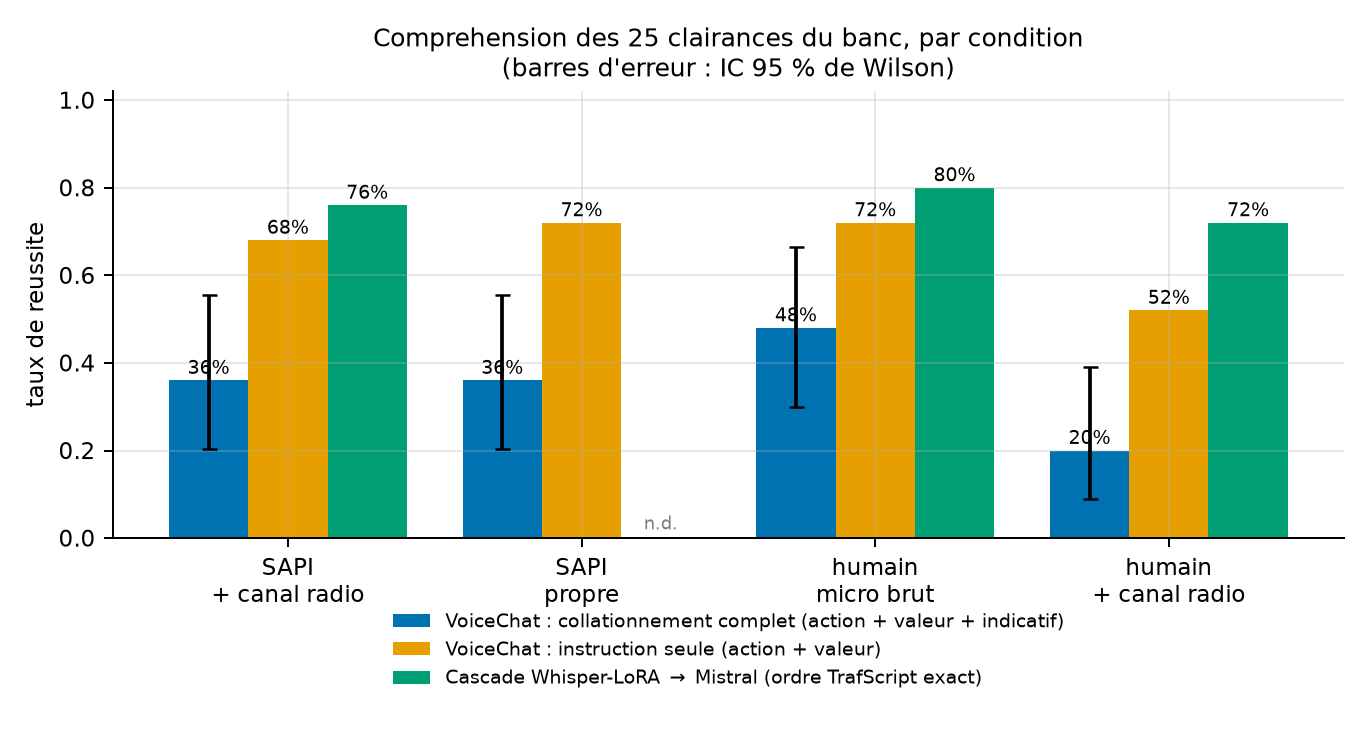
\includegraphics[width=0.94\textwidth]{figures/fig_voicechat_conditions.png}
\caption{Taux de réussite par condition. En bleu le collationnement complet, en
orange l'instruction seule (indicatif ignoré), en vert la référence de la
cascade sur exactement les mêmes énoncés. La condition « SAPI propre » n'a pas
d'équivalent dans les campagnes antérieures.}
\label{fig:conditions}
\end{figure}

\begin{table}[h]
\centering
\caption{Résultats détaillés par condition. Les intervalles de confiance sont
ceux de Wilson~\cite{wilson} à 95\,\%, adaptés aux petits effectifs. Le WER de collationnement
mesure l'écart mot à mot avec le collationnement canonique attendu.}
\label{tab:resultats}
\small
\setlength{\tabcolsep}{4.5pt}
\begin{tabular}{@{}lccccc@{}}
\toprule
\textbf{Condition} & \textbf{Collationnement} & \textbf{IC 95\,\%} &
\textbf{Instruction seule} & \textbf{WER collat.} & \textbf{Latence méd.}\\
\midrule
\texttt{sapi\_radio}   & 9/25 = 36\,\%  & [0,20 ; 0,55] & 17/25 = 68\,\% & 0,85 & 30,9\,s\\
\texttt{sapi\_propre}  & 9/25 = 36\,\%  & [0,20 ; 0,55] & 18/25 = 72\,\% & 1,03 & 30,8\,s\\
\texttt{humain\_micro} & 12/25 = 48\,\% & [0,30 ; 0,67] & 18/25 = 72\,\% & 0,97 & 37,0\,s\\
\texttt{humain\_radio} & 5/25 = 20\,\%  & [0,09 ; 0,39] & 13/25 = 52\,\% & 1,92 & 37,3\,s\\
\bottomrule
\end{tabular}
\end{table}

Deux observations se dégagent de ce tableau. La première concerne l'effet du
canal radio, et elle est contre-intuitive : la dégradation ne coûte presque rien
sur la voix de synthèse, qui reste à 36\,\% avec ou sans, mais elle coûte plus
de la moitié du score sur la voix humaine, qui tombe de 48\,\% à 20\,\%. Le
modèle encaisse donc mal le \emph{cumul} d'un accent, d'une prosodie naturelle et
d'un canal dégradé, là où chacun de ces facteurs pris isolément lui pose peu de
problème. C'est exactement l'avertissement que porte la carte du modèle sur les
environnements bruités, et il se vérifie ici sur nos propres données. La seconde
observation est qu'une seule réponse sur cent est restée muette : le modèle
\emph{répond} presque toujours, et ce n'est donc pas sa disponibilité qui est en
cause mais le contenu de ce qu'il dit.

Reste à savoir si cet écart avec la cascade est réel ou s'il pourrait tenir au
hasard de l'échantillon. C'est l'objet du test apparié décrit plus haut, dont le
tableau~\ref{tab:mcnemar} donne les résultats.

\begin{table}[h]
\centering
\caption{Comparaisons appariées avec la cascade (test exact de McNemar, seuils
corrigés par la méthode de Holm). $n_{01}$ compte les énoncés que VoiceChat
réussit et que la cascade manque ; $n_{10}$ l'inverse.}
\label{tab:mcnemar}
\small
\begin{tabular}{@{}lccccc@{}}
\toprule
\textbf{Comparaison} & \textbf{VoiceChat} & \textbf{Cascade} &
$n_{01}$ & $n_{10}$ & $p_{\text{Holm}}$\\
\midrule
\texttt{sapi\_radio} vs cascade ROMEO  & 9/25  & 19/25 & 0 & 10 & \textbf{0,006}\\
\texttt{sapi\_radio} vs cascade locale & 9/25  & 19/25 & 0 & 10 & \textbf{0,006}\\
\texttt{humain\_micro} vs cascade      & 12/25 & 20/25 & 0 & 8  & \textbf{0,008}\\
\texttt{humain\_radio} vs cascade      & 5/25  & 18/25 & 0 & 13 & \textbf{0,001}\\
\bottomrule
\end{tabular}
\end{table}

Une lecture par énoncé complète ce tableau. Sur les 25 clairances, 3 seulement
sont réussies dans les quatre conditions et 6 ne le sont dans aucune : le corpus
comporte donc un noyau d'énoncés que le modèle traite de façon stable, un noyau
qu'il manque systématiquement, et une majorité de cas dont l'issue dépend de la
voix et du canal. Cette instabilité est en soi une information : elle indique que
le modèle n'a pas de représentation robuste de la tâche, et que ses réussites
tiennent en partie aux conditions d'écoute.

Les quatre probabilités sont inférieures à 0,01 : l'écart est établi. Mais le
résultat le plus instructif n'est pas là, il est dans la colonne $n_{01}$, qui
vaut zéro dans les quatre comparaisons. Rappelons ce que compte cette colonne :
le nombre d'énoncés que VoiceChat a réussis alors que la cascade les manquait.
Il n'y en a aucun. \textbf{VoiceChat n'a jamais rattrapé un échec de la
cascade.} Sa performance n'est donc pas seulement inférieure, elle est
\emph{strictement incluse} dans celle de la chaîne existante. La conséquence est
importante pour la suite du projet : il n'y a rien à gagner à combiner les deux
approches, puisque le modèle bout-en-bout n'apporte aucun cas que la cascade ne
traite déjà.

\subsection{Deux échecs structurels : l'outil muet et l'indicatif}
\label{sec:outils}

Le premier échec est le plus lourd de conséquences. Sur les 100 stimuli de la
campagne, et sur toutes les variantes d'invite essayées pendant la calibration,
le canal d'appel d'outils est resté vide. Pas une seule fois le modèle n'a émis
la commande structurée que le simulateur attend. Il faut prendre la mesure de ce
que signifie un zéro sur cent : l'intervalle de confiance de Wilson associé
place la vraie proportion d'appels d'outil sous 3,7\,\%, ce qui exclut
l'hypothèse d'un déclenchement simplement rare que la campagne aurait manqué par
malchance. Cela retire au modèle
bout-en-bout sa raison d'être dans notre architecture : puisque seule sa parole
est exploitable, il faudrait de toute façon lui adjoindre un analyseur pour
convertir ce qu'il dit en ordre exécutable, et l'on retomberait sur une cascade
« VoiceChat vers analyseur ». L'économie d'étages, qui était l'argument de
départ, disparaît.

Ce silence est cohérent avec les limites que NVIDIA publie : une précision des
arguments de 44,2\,\% seulement, l'incapacité à appeler plusieurs outils
simultanément, et la mention explicite que « dans les conversations mixtes, le
modèle peut répondre depuis ses propres connaissances au lieu d'appeler l'outil
approprié ». S'y ajoute, de notre côté, la contrainte de trames identifiée à la
section précédente, qui rend les invites d'appel d'outils inutilisables sur des
énoncés de quelques secondes : l'invite officielle est si longue qu'elle ne
laisse plus au modèle aucune trame pour produire quoi que ce soit.

Le second échec touche le contenu de la parole, et il a une structure très nette.
La figure~\ref{fig:echecs} décompose les collationnements erronés selon le
constituant qui manque, et le même constituant domine dans les quatre
conditions : l'indicatif.

\begin{figure}[h]
\centering
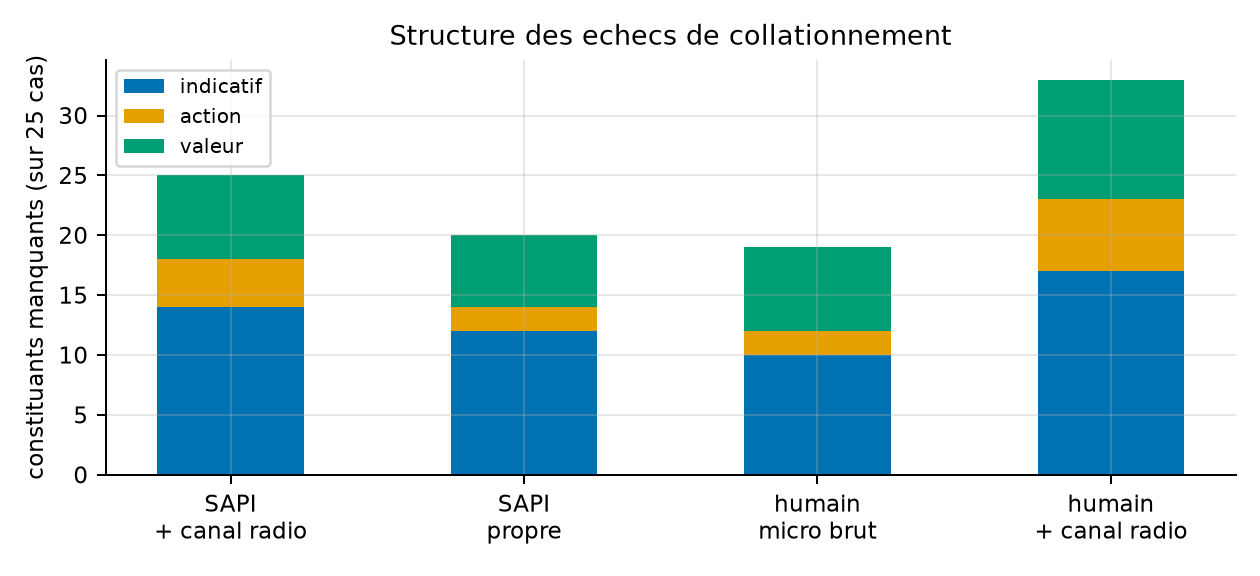
\includegraphics[width=0.8\textwidth]{figures/fig_voicechat_echecs.png}
\caption{Constituants manquants dans les collationnements erronés. L'indicatif
domine dans les quatre conditions.}
\label{fig:echecs}
\end{figure}

Le tableau~\ref{tab:parindicatif} pousse l'analyse un cran plus loin, en
donnant le taux de reconnaissance indicatif par indicatif. La hiérarchie qu'il
révèle est sans ambiguïté.

\begin{table}[h]
\centering
\caption{Taux de reconnaissance de l'indicatif, indicatif par indicatif, sur les
quatre conditions cumulées. La colonne de droite donne la forme que la
phraséologie impose de prononcer.}
\label{tab:parindicatif}
\small
\begin{tabular}{@{}lcl@{}}
\toprule
\textbf{Indicatif} & \textbf{Reconnu} & \textbf{Forme parlée attendue}\\
\midrule
\texttt{AFR1234} & 31/40 = 78\,\% & \emph{air france one two three four}\\
\texttt{DLH88}   & 3/8 \ = 38\,\% & \emph{lufthansa eight eight}\\
\texttt{BAW57}   & 8/24 = 33\,\% & \emph{speedbird five seven}\\
\texttt{EZY21}   & 3/12 = 25\,\% & \emph{easyjet two one}\\
\texttt{RYR9}    & 2/8 \ = 25\,\% & \emph{ryanair niner}\\
\texttt{CSA1DZ}  & \textbf{0/8 \ = 0\,\%} & \emph{c s a one delta zulu}\\
\bottomrule
\end{tabular}
\end{table}

L'indicatif le mieux reconnu, et de loin, est celui qui ressemble le plus à de
l'anglais ordinaire : \emph{air france} suivi de quatre chiffres, reconnu dans
78\,\% des cas. À l'autre extrémité, l'indicatif \texttt{CSA1DZ}, qui exige
l'alphabet radio (\emph{c s a one delta zulu}), n'est \textbf{jamais} reconnu,
pas une seule fois sur huit essais. Entre les deux, les indicatifs de compagnie
peu courants dans la langue générale, \emph{speedbird} ou \emph{ryanair},
plafonnent autour de 30\,\%. Le modèle réussit donc là où la phraséologie
ressemble à de l'anglais, et échoue exactement là où elle s'en écarte : c'est la
signature d'un modèle qui n'a jamais rencontré ce domaine pendant son
entraînement, et non d'un modèle qui entend mal.

Le chiffre le plus parlant reste que \textbf{31 cas sur 100} présentent une
instruction parfaitement comprise et un indicatif faux. Le modèle entend correctement le cap
ou le niveau de vol, mais se trompe sur l'identité de l'avion auquel il répond,
ce qui rend l'ordre inutilisable en pratique et dangereux en principe. Le
tableau~\ref{tab:indicatifs} en donne des exemples caractéristiques.

\begin{table}[h]
\centering
\caption{Exemples de collationnements produits, avec l'ordre attendu en regard.
Les erreurs portent sur l'indicatif et sur les nombres épelés.}
\label{tab:indicatifs}
\small
\begin{tabular}{@{}ll@{}}
\toprule
\textbf{Attendu} & \textbf{Collationnement produit}\\
\midrule
\texttt{HDG EZY21 100}   & « \emph{Y two hundred one fly heading one hundred} »\\
\texttt{HDG BAW57 310}   & « \emph{Beware five seven turn left heading three hundred and ten} »\\
\texttt{ALT CSA1DZ 24000}& « \emph{Climb flight level two four zero, Delta Zulu} »\\
\texttt{ALT BAW57 8000}  & « \emph{Descend to flight level eighty, C-A-W-U five thousand seven hundred} »\\
\texttt{HDG DLH88 180}   & « \emph{Lutana eight heading one hundred and eighty zero} »\\
\texttt{ALT AFR1234 32000}& « \emph{Climb flight level three hundred and twenty zero} »\\
\bottomrule
\end{tabular}
\end{table}

La lecture de ces exemples est éclairante. « \emph{Speedbird} », l'indicatif
radio de British Airways, devient « \emph{Beware} » ou « \emph{C-A-W-U} » ;
« \emph{lufthansa} » devient « \emph{Lutana} » ; et le niveau de vol 320,
qui s'épelle « \emph{three two zero} » en phraséologie, devient « \emph{three
hundred and twenty zero} ». Le modèle ne fait pas n'importe quoi : il
« naturalise » systématiquement, c'est-à-dire qu'il ramène ce qu'il entend vers
l'anglais courant qu'il connaît, faute d'avoir jamais rencontré la phraséologie
aéronautique pendant son entraînement. Ce sont précisément les erreurs qu'un
modèle généraliste commet par manque d'exposition au domaine, et précisément
celles que notre adaptation LoRA sur corpus ATC a corrigées dans l'étage de
reconnaissance vocale.

Un troisième type d'échec, plus discret, mérite d'être signalé parce qu'il est
le plus dangereux des trois. Dans onze cas sur cent, l'action et l'indicatif
sont tous deux corrects, et c'est la \emph{valeur} qui est fausse : le bon avion
reçoit le bon type d'ordre, mais pas le bon nombre. Un collationnement de ce
genre est plausible à l'oreille et passerait sans alerter un contrôleur pressé,
alors qu'un indicatif manifestement absurde se remarque immédiatement. Dans notre
architecture, ces cas seraient de toute façon interceptés en aval par la
validation déterministe, qui contrôle les bornes physiques ; c'est précisément
la fonction de cette couche, et cette campagne en fournit une illustration
supplémentaire.

Enfin, quatre réponses sur cent sortent complètement du rôle de pilote et
répondent en assistant conversationnel, par exemple en expliquant ce qu'est une
clairance au lieu de la collationner. Ce comportement, marginal ici, rappelle
que le modèle reste un assistant généraliste que l'invite système contraint
imparfaitement.

\subsection{Ce que le modèle réussit : la voix, et à quel prix}

Le tableau du modèle n'est pas uniformément sombre, et son point fort se situe
là où on ne l'attendait pas nécessairement : la qualité de la voix qu'il produit.
La figure~\ref{fig:tts} le compare aux moteurs de synthèse déjà mesurés dans le
projet, selon le protocole habituel du banc : on fait prononcer un texte par le
moteur, on redonne l'enregistrement à un système de reconnaissance vocale fixe
qui joue le rôle de juge, et l'on mesure l'écart entre ce que le juge a
retranscrit et le texte de départ. Plus cet écart est faible, plus la voix est
intelligible.

\begin{figure}[h]
\centering
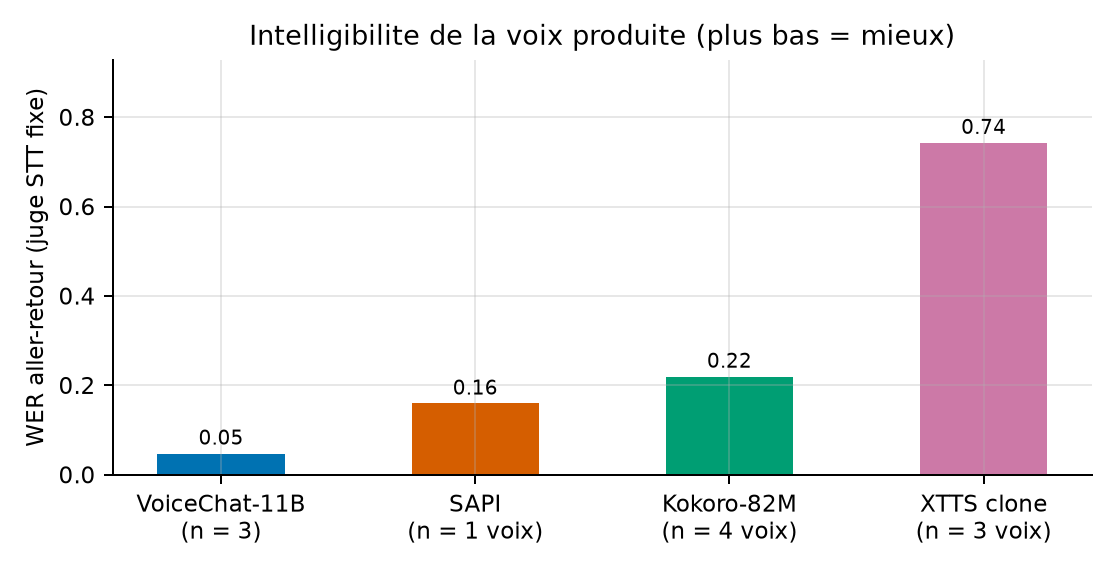
\includegraphics[width=0.72\textwidth]{figures/fig_voicechat_tts.png}
\caption{Intelligibilité aller-retour (synthèse, puis juge STT fixe, puis WER),
protocole \texttt{tts\_bench}. Plus bas est meilleur.}
\label{fig:tts}
\end{figure}

Le résultat est net : le juge retranscrit la parole de VoiceChat presque mot pour
mot, avec un écart de \textbf{0,048}, contre 0,16 pour la voix système SAPI,
0,22 en moyenne pour Kokoro-82M et 0,74 pour les voix XTTS clonées que nous
utilisons sur ROMEO. La voix du modèle bout-en-bout est donc la plus intelligible
de toutes celles mesurées dans le projet. Deux réserves de méthode s'imposent
néanmoins, et il vaut mieux les énoncer soi-même : le sous-échantillon décodé en
audio ne compte que trois énoncés, ce qui est peu ; et ce chiffre suppose une
correction de format appliquée au juge, qui écrit « 1-2-3-4 » là où le modèle dit
« \emph{one two three four} ». Sans cette fusion des chiffres tiretés, le score
affiché serait de 0,71 alors même que la transcription est correcte mot pour mot.
Les moteurs de référence ayant été mesurés sans cette correction, la comparaison
est indicative plutôt que rigoureusement homogène.

Ce résultat a toutefois un prix, qu'il faut mettre en regard. Le chargement du
modèle prend de 162 à 166\,s, pour un checkpoint de 44,4\,Go ; le modèle
s'exécute en \texttt{float32} et occupe 44,5\,Go de mémoire graphique. Le passage
en demi-précision (\texttt{bfloat16}) le ramènerait à 22,3\,Go, mais casse le
décodeur de synthèse, dont les types sont mixtes. Quant à la génération, elle
tourne à un \textbf{facteur temps réel d'environ 3}, c'est-à-dire qu'il faut
trois secondes de calcul pour produire une seconde de parole : 32\,s pour 10,8\,s
d'audio. Le décodage audio, lui, coûte peu : 32,7\,s avec contre 31,9\,s sans,
soit 0,9\,s de plus, moins de 3\,\% du temps total. À titre de comparaison, la cascade complète répond en 8,4\,s de
médiane sur le même calculateur, et en 2,5\,s sur un poste local.

Une précaution d'interprétation s'impose sur ces durées. Elles mesurent le
chemin de référence NeMo utilisé hors ligne pour l'évaluation, et non le moteur
d'inférence temps réel que NVIDIA annonce à 448\,ms de prise de parole. Elles
quantifient donc le coût d'une \emph{campagne de mesure}, pas une latence
déployable en salle de simulation.

\subsection{Une capacité que notre cascade n'a pas : l'interruption de parole}

Parmi les démonstrations publiées par NVIDIA figure un comportement que notre
chaîne ne sait pas reproduire : l'\emph{interruption}, ou \emph{barge-in}.
L'utilisateur se met à parler pendant que l'agent parle ; l'agent s'arrête net,
au milieu d'un mot, et enchaîne sur ce qu'on vient de lui dire. Comme cette
capacité est souvent citée comme l'argument décisif des modèles full-duplex, il
vaut la peine de regarder précisément ce que notre architecture permet, et pour
quelle raison.

La vérification est sans appel : notre chaîne est \textbf{half-duplex par
construction}, et trois points du code l'établissent. D'abord, le micro
n'écoute que pendant que la touche d'alternat est maintenue : dans
\texttt{RadioPanel.tsx}, la capture s'ouvre à l'appui sur la touche et se ferme
au relâchement, moment auquel seulement l'enregistrement part vers l'API de
reconnaissance. Pendant que le pilote virtuel parle, rien n'écoute. Ensuite,
l'audio du collationnement est techniquement injoignable : la fonction
\texttt{playB64Wav} de \texttt{audio.ts} crée l'objet \texttt{Audio} dans une
variable locale et le lit sans en conserver de référence, si bien qu'il n'existe
nulle part dans l'interface de quoi l'arrêter. Enfin, la boucle est strictement
séquentielle, de la capture à la lecture en passant par la transcription,
l'interprétation, la validation et la synthèse : chaque étage attend que le
précédent ait terminé, et aucune détection d'activité vocale ne tourne pendant
la lecture.

Cette limite est réelle, mais il serait faux d'en faire un défaut, et c'est le
point le plus important de cette section. \textbf{La radiotéléphonie
aéronautique est elle-même half-duplex} : sur une fréquence VHF, un seul
émetteur peut parler à la fois, et deux transmissions simultanées se brouillent
mutuellement, ce que la phraséologie appelle une \emph{transmission bloquée}.
Notre alternat au clavier reproduit donc fidèlement la contrainte du métier,
tandis que le barge-in de VoiceChat est un comportement d'assistant
conversationnel, emprunté au dialogue humain ordinaire, et non à la
radiotéléphonie. Autrement dit, la capacité qui impressionne le plus dans la
démonstration du modèle est celle dont notre cas d'usage a le moins besoin. Le
half-duplex est ici un choix de conception assumé, pas une limite subie.

Il reste qu'un demi-pas serait peu coûteux et améliorerait l'ergonomie. Il
suffirait de conserver une référence à l'objet audio en cours de lecture et de
l'arrêter à l'appui sur la touche d'alternat, soit une quinzaine de lignes, pour
obtenir un \emph{barge-in manuel} : l'élève reprend la fréquence et le pilote se
tait immédiatement, exactement comme un contrôleur qui reprend l'alternat. Cela
ne donnerait pas l'interruption automatique détectée à la voix, qui suppose
d'écouter et de parler simultanément et donc de changer d'architecture, mais
cela supprimerait le cas gênant où il faut attendre la fin d'un collationnement
pour pouvoir répondre.

%=============================================================================
\section{Conclusion et perspectives}
%=============================================================================

\textbf{En l'état, ce modèle ne peut pas remplacer la cascade du projet.} Il
s'agit d'un assistant conversationnel généraliste : il entend correctement
l'instruction (environ 70\,\% hors bruit) mais échoue sur ce qui constitue le
cœur du domaine, à savoir les indicatifs OACI et les nombres épelés, et n'émet aucun
ordre structuré exploitable par le simulateur. L'écart avec la chaîne existante
est statistiquement établi, et sa performance est strictement incluse dans celle
de la cascade.

Un résultat négatif reste un résultat, et celui-ci est instructif pour la suite
du projet à trois titres.

Il valide d'abord, empiriquement, notre choix d'affiner la reconnaissance
vocale. Les erreurs commises par ce modèle généraliste, « \emph{Beware five
seven} » pour \emph{speedbird five seven} ou « \emph{Lutana eight} » pour
\emph{lufthansa eight}, sont exactement celles que notre adaptateur LoRA entraîné
sur corpus ATC corrige dans l'étage de reconnaissance. Nous disposons donc d'une
justification externe, obtenue sur un modèle tiers que nous n'avons pas
construit, d'une décision d'architecture prise en semaine 4 du stage. C'est
une confirmation d'autant plus solide qu'elle ne vient pas de nos propres
mesures.

Il indique ensuite où se situe la marge de progression de l'approche
bout-en-bout, et elle n'est pas là où on l'imaginerait. La synthèse vocale du
modèle surclasse nettement celle que nous utilisons, et son canal d'appel
d'outils, s'il était activé par un affinage sur des clairances aéronautiques,
supprimerait entièrement l'étage d'interprétation. La barrière n'est donc pas
architecturale : rien dans la conception du modèle n'interdit qu'il fasse le
travail. Elle tient à l'absence d'exposition au domaine, ce qui est un problème
de données, pas de structure, et donc un problème soluble.

Il documente enfin une contrainte peu connue des modèles full-duplex synchrones
à la trame, que nous n'avons trouvée mentionnée nulle part : l'invite système et
le temps de parole disponible puisent dans le même budget de génération. Toute
évaluation future de ce type de modèle doit en tenir compte, sous peine de
mesurer un silence et de conclure à tort à une incapacité du modèle. C'est
peut-être l'apport le plus réutilisable de cette note.

Une suite naturelle, si le calendrier l'avait permis, aurait été d'affiner
VoiceChat sur les corpus ATCO2~\cite{atco2} et UWB-ATCC déjà utilisés dans le
projet, puis de
rejouer exactement ce protocole pour mesurer l'écart. Les scripts, les stimuli et
la vérité terrain sont conservés et réutilisables tels quels, de sorte que cette
comparaison reste ouverte à quiconque voudra la mener.

%=============================================================================
\clearpage
\renewcommand{\refname}{Références}
\addcontentsline{toc}{section}{Références}
%=============================================================================

\begin{thebibliography}{99}\small

\bibitem{voicechat11b} NVIDIA (NemotronLabs),
\emph{NVIDIA-NemotronLabs-VoiceChat-11B}, carte de modèle, licence
OpenMDW 1.1, 3 août 2026.
\url{https://huggingface.co/nvidia/NVIDIA-NemotronLabs-VoiceChat-11B}

\bibitem{casanova2025asru} E.~Casanova, C.~Chen, K.~Hu, A.~Pasad,
E.~Rastorgueva, S.~Lakshmi Narasimhan, S.~Deng, E.~Hosseini-Asl, P.~Żelasko,
V.~Mendelev, S.~Ghosh, Y.~Peng, Z.~Chen, J.~Li, J.~Balam, V.~Lavrukhin et
B.~Ginsburg, « Open Full-duplex Voice Agent with Speech-to-Speech Language
Model », \emph{IEEE Automatic Speech Recognition and Understanding Workshop
(ASRU)}, Honolulu, p.~1--4, 2025. doi:10.1109/ASRU65441.2025.11434669

\bibitem{salmduplex} K.~Hu, E.~Hosseini-Asl, C.~Chen, E.~Casanova, S.~Ghosh,
P.~Żelasko, Z.~Chen, J.~Li, J.~Balam et B.~Ginsburg, « Efficient and Direct
Duplex Modeling for Speech-to-Speech Language Model », \emph{Interspeech},
ISCA, p.~2715--2719, 2025. doi:10.21437/Interspeech.2025-874

\bibitem{fullduplexbench} G.-T.~Lin, J.~Lian, T.~Li, Q.~Wang,
G.~Anumanchipalli, A.~H.~Liu et H.-y.~Lee, « Full-Duplex-Bench: A Benchmark to
Evaluate Full-duplex Spoken Dialogue Models on Turn-taking Capabilities »,
\emph{IEEE Automatic Speech Recognition and Understanding Workshop (ASRU)},
p.~1--8, 2025. doi:10.1109/ASRU65441.2025.11433838

\bibitem{fullduplexbenchv3} G.-T.~Lin, C.~Chen, Z.~Chen et H.-y.~Lee,
« Full-Duplex-Bench-v3: Benchmarking Tool Use for Full-Duplex Voice Agents
Under Real-World Disfluency », prépublication arXiv:2604.04847, 2026.
(Travail annoncé comme en cours : aucune version publiée à ce jour.)

\bibitem{nemotronnano2} NVIDIA, « NVIDIA Nemotron Nano 2: An Accurate and
Efficient Hybrid Mamba-Transformer Reasoning Model », rapport technique,
prépublication arXiv:2508.14444, 2025. (Rapport collectif ; l'auteur déclaré
est l'organisation.)

\bibitem{mamba2} T.~Dao et A.~Gu, « Transformers are SSMs: Generalized Models
and Efficient Algorithms Through Structured State Space Duality »,
\emph{Proc. 41st International Conference on Machine Learning (ICML)}, PMLR
vol.~235, p.~10041--10071, 2024.

\bibitem{fastconformer} D.~Rekesh, N.~R.~Koluguri, S.~Kriman, S.~Majumdar,
V.~Noroozi, H.~Huang, O.~Hrinchuk, K.~Puvvada, A.~Kumar, J.~Balam et
B.~Ginsburg, « Fast Conformer with Linearly Scalable Attention for Efficient
Speech Recognition », \emph{IEEE Automatic Speech Recognition and
Understanding Workshop (ASRU)}, Taipei, p.~1--8, 2023.
doi:10.1109/ASRU57964.2023.10389701

\bibitem{whisper} A.~Radford, J.~W.~Kim, T.~Xu, G.~Brockman, C.~McLeavey et
I.~Sutskever, « Robust Speech Recognition via Large-Scale Weak Supervision »,
\emph{Proc. 40th International Conference on Machine Learning (ICML)}, PMLR
vol.~202, p.~28492--28518, 2023.

\bibitem{lora} E.~J.~Hu, Y.~Shen, P.~Wallis, Z.~Allen-Zhu, Y.~Li, S.~Wang,
L.~Wang et W.~Chen, « LoRA: Low-Rank Adaptation of Large Language Models »,
\emph{International Conference on Learning Representations (ICLR)}, 2022.

\bibitem{atco2} J.~P.~Zuluaga-Gomez, K.~Veselý, I.~Szöke, A.~Blatt,
P.~Motlicek, M.~Kocour, K.~Choukri, I.~Nigmatulina, C.~Cevenini, A.~Tart,
J.~Černocký et D.~Klakow, « ATCO2 corpus: A Large-Scale Dataset for Research
on Automatic Speech Recognition and Natural Language Understanding of Air
Traffic Control Communications », \emph{Journal of Data-centric Machine
Learning Research}, vol.~2, article~5, p.~1--45, 2024.

\bibitem{bluesky} J.~M.~Hoekstra et J.~Ellerbroek, « BlueSky ATC Simulator
Project: an Open Data and Open Source Approach », \emph{7th International
Conference on Research in Air Transportation (ICRAT)}, Philadelphie, 2016.

\bibitem{mcnemar} Q.~McNemar, « Note on the Sampling Error of the Difference
Between Correlated Proportions or Percentages », \emph{Psychometrika},
vol.~12, n\textsuperscript{o}~2, p.~153--157, 1947. doi:10.1007/BF02295996

\bibitem{holm} S.~Holm, « A Simple Sequentially Rejective Multiple Test
Procedure », \emph{Scandinavian Journal of Statistics}, vol.~6,
n\textsuperscript{o}~2, p.~65--70, 1979.
(Antérieur au système DOI ; référence stable JSTOR 4615733.)

\bibitem{wilson} E.~B.~Wilson, « Probable Inference, the Law of Succession,
and Statistical Inference », \emph{Journal of the American Statistical
Association}, vol.~22, n\textsuperscript{o}~158, p.~209--212, 1927.
doi:10.1080/01621459.1927.10502953

\end{thebibliography}

%=============================================================================
\section*{Annexe : reproductibilité}
\addcontentsline{toc}{section}{Annexe : reproductibilité}
%=============================================================================

Tous les chiffres de \emph{résultats} de cette note (taux de réussite,
intervalles de confiance, probabilités, WER, latences, facteur temps réel)
proviennent des fichiers du banc, \texttt{voicechat\_romeo.json} et le dossier
\texttt{voicechat\_audio/} dans \texttt{bench/results/}, et les figures sont
produites par \texttt{gen\_figures.py} à partir de ces mêmes fichiers. Trois
catégories de valeurs font exception et sont d'une autre nature : les
caractéristiques annoncées du modèle (latence, précision d'appel d'outil,
taille), qui proviennent de sa carte de modèle~\cite{voicechat11b} ; les
chiffres d'exploitation du calculateur (quotas, occupation mémoire, durées de
compilation), relevés dans le journal de déploiement ; et le tableau de
calibration des invites, dont seule la variante retenue a été conservée dans
les livrables. Ces valeurs sont signalées comme telles dans le texte.

La campagne se rejoue en six étapes, dans l'ordre des commandes ci-dessous. La
première prépare localement les stimuli, soit quatre conditions de vingt-cinq
clairances. La deuxième réserve un nœud de ROMEO et y installe l'environnement
et le checkpoint, entièrement sur le disque RAM. La troisième y transfère les
stimuli. La quatrième lance la campagne complète, environ une heure pour cent
stimuli, puis le sous-échantillon décodé en audio. La cinquième rapatrie les
sorties et calcule les scores localement, avec le code de production du dépôt.
La sixième libère le nœud.

\begin{lstlisting}[language=bash]
bench/bench-env/Scripts/python.exe bench/voicechat/prepare_stimuli.py

tr -d '\r' < bench/voicechat/job_setup.slurm | ssh romeo sbatch

scp bench/results/voicechat_stimuli/stimuli.tar.gz romeo:/tmp/
ssh romeo 'sbcast -j <jobid> -f /tmp/stimuli.tar.gz /dev/shm/vc/stimuli.tar.gz'

ssh romeo 'srun --jobid=<jobid> --overlap bash /dev/shm/vc/run_campaign.sh complet'
ssh romeo 'srun --jobid=<jobid> --overlap bash /dev/shm/vc/run_audio_subset.sh 3'

bash bench/voicechat/pull_results.sh <jobid> complet bench/results/voicechat_raw
bench/bench-env/Scripts/python.exe bench/voicechat_bench.py

ssh romeo 'scancel --name=vc-setup'
\end{lstlisting}

\noindent
\textbf{Inventaire.} \texttt{bench/voicechat/} (scripts SLURM, stimuli,
inférence côté cluster, contournements ROMEO) ;
\texttt{bench/voicechat\_bench.py} (scoring et statistiques) ;
\texttt{bench/results/} (résultats détaillés et parole produite) ;
\texttt{rapport\_voicechat/} (cette note). \emph{Test exploratoire : aucun
livrable existant n'a été modifié.}

\end{document}
